%% This is file `elsarticle-template-1-num.tex',
%%
%% Copyright 2009 Elsevier Ltd
%%
%% This file is part of the 'Elsarticle Bundle'.
%% ---------------------------------------------
%%
%% It may be distributed under the conditions of the LaTeX Project Public
%% License, either version 1.2 of this license or (at your option) any
%% later version.  The latest version of this license is in
%%    http://www.latex-project.org/lppl.txt
%% and version 1.2 or later is part of all distributions of LaTeX
%% version 1999/12/01 or later.
%%
%% Template article for Elsevier's document class `elsarticle'
%% with numbered style bibliographic references
%%
%% $Id: elsarticle-template-1-num.tex 149 2009-10-08 05:01:15Z rishi $
%% $URL: http://lenova.river-valley.com/svn/elsbst/trunk/elsarticle-template-1-num.tex $
%%
%\documentclass[preprint,12pt]{elsarticle}
\documentclass{article}

%% Use the option review to obtain double line spacing
%% \documentclass[preprint,review,12pt]{elsarticle}

%% Use the options 1p,twocolumn; 3p; 3p,twocolumn; 5p; or 5p,twocolumn
%% for a journal layout:
%% \documentclass[final,1p,times]{elsarticle}
%% \documentclass[final,1p,times,twocolumn]{elsarticle}
%% \documentclass[final,3p,times]{elsarticle}
%% \documentclass[final,3p,times,twocolumn]{elsarticle}
%% \documentclass[final,5p,times]{elsarticle}
%% \documentclass[final,5p,times,twocolumn]{elsarticle}

%% The graphicx package provides the includegraphics command.
\usepackage{graphicx}
%% The amssymb package provides various useful mathematical symbols
\usepackage{amssymb}
%% The amsthm package provides extended theorem environments
%% \usepackage{amsthm}
\usepackage{amsmath}
\usepackage{multicol}

\usepackage{todonotes}
\usepackage{float}
\usepackage{booktabs}
\usepackage{subfig}

%% The lineno packages adds line numbers. Start line numbering with
%% \begin{linenumbers}, end it with \end{linenumbers}. Or switch it on
%% for the whole article with \linenumbers after \end{frontmatter}.
\usepackage{lineno}

%% natbib.sty is loaded by default. However, natbib options can be
%% provided with \biboptions{...} command. Following options are
%% valid:

%%   round  -  round parentheses are used (default)
%%   square -  square brackets are used   [option]
%%   curly  -  curly braces are used      {option}
%%   angle  -  angle brackets are used    <option>
%%   semicolon  -  multiple citations separated by semi-colon
%%   colon  - same as semicolon, an earlier confusion
%%   comma  -  separated by comma
%%   numbers-  selects numerical citations
%%   super  -  numerical citations as superscripts
%%   sort   -  sorts multiple citations according to order in ref. list
%%   sort&compress   -  like sort, but also compresses numerical citations
%%   compress - compresses without sorting
%%
%% \biboptions{comma,round}

% \biboptions{}

%\journal{Journal Name}

\title{TREMA-UNH at TREC 2018: Complex Answer Retrieval and News Track}


\author{Sumanta Kashyapi, Shubham Chatterjee, Jordan Ramsdell, Laura Dietz \\
\texttt{\{sk1105, sc1242, jsc57\}@wildcats.unh.edu, dietz@cs.unh.edu}\\
TREMA lab, University of New Hampshire, U.S.A}
\date{} 

\begin{document}

\maketitle 
%% Title, authors and addresses

\begin{abstract}
This notebook describes the submission of team TREMA-UNH to the TREC Complex Answer Retrieval track and the TREC News track in 2018. Our methods focus on passage retrieval, entity-aware passage retrieval, and entity retrieval.
\end{abstract}




%%
%% Start line numbering here if you want
%%

%% main text
\section{Introduction}
\label{S:1}

Search engines continue to develop and so do the users' expectations of it. We explore ``search engines of the future'' that are not only presenting a ranking of top documents but present all relevant information in a compact manner from which users are able to synthesize knowledge easily. Moreover, the goal is to develop search engines to understand their information need more accurately and retrieve documents pertaining to their needs. To accomplish these tasks, we train the search engines to have a better understanding of natural language. 

The Complex Answer Retrieval (CAR)\cite{dietztrec} track at the Text Retrieval Conference (TREC)\footnote{\url{https://trec.nist.gov}} aims to address this scenario. Current retrieval systems provide good solutions towards phrase-level retrieval for simple fact and entity-centric needs. This track encourages research for answering more complex information needs with longer answers.
The formal task statement includes the two following tasks:

\noindent \textbf{Passage Task:} Given an article stub $Q$, retrieve for each of its sections $H_i$, a ranking of relevant passages $P$. The passage $P$ is taken from a provided passage corpus.

\noindent \textbf{Entity Task:} Given an article stub $Q$, retrieve for each of its sections $H_i$, a ranking of relevant entities $E$. The entity $E$ is taken from a provided Wikipedia corpus. Additionally for each entity $E$, a support passage from the passage corpus is to be identified that explains why the entity is relevant for the heading $H_i$ on the stub.
\medskip

\noindent We further participate in the NEWS track entity ranking task. 

\noindent \textbf{NEWS Entity Task:} Given a news article with title and content that is annotated with entity links to a set of entities  $\mathcal{E}=\{E1, E2, ... En\}$, the task is to rank the the given entities by importance for the article (i.e., saliency). 

\medskip 

\section{Overarching Approach}
The queries provided to us contains an outline for each page. We use the section headings from each outline as our queries. However, the headings are usually very short. Hence, using retrieval models without expansion (such as BM25) may not yield good results since headings have little textual overlap with their passages. To alleviate this problem, we experiment with various query expansion methods. We observe the performance of each of the methods individually. However, as any single unsupervised methods may not provide best performance on its own. Hence, we also experiment with a machine-learned combination of each of the models using learning-to-rank. 

The Knowledge Graph is a knowledge base used to enhance a search engine's results with information gathered from a variety of sources. It provides access to sophisticated knowledge about entities derived from external sources such as Wikipedia. Such knowledge graphs hold a wealth of information which can be leveraged to solve information retrieval problems. 

In Section \ref{sec:para} we will first describe which unsupervised retrieval and expansion models were used for paragraph retrieval, and in Section \ref{sec:entity} for entity retrieval.  

%This was already said above.
%The section headings and paragraphs in the TREC-CAR dataset are not generated from the same model. Section headings are constructed in such a way that they best capture the prevalent ideas expressed in the paragraphs under them. Conversely, paragraphs could be seen as elaboration of the the section heading. Hence, for the passage retrieval task, there is little chance of success if we try to directly map section headings to paragraph texts. Hence, we try to estimate the language model over top-k TF-IDF words of the feedback run and use it to map paragraphs to section headings.


%\section{Related Work and Background}
%\label{S:2}
\section{Low-level Retrieval Features}

Each of our approaches are based on (a subset of) a variety of unsupervised retrieval models and indexes we describe in the following.

\paragraph{Indexes:}

We create different search indexes. 
\begin{itemize}
    \item A paragraph index out the text in passages of the \texttt{paragraphCorpus}.
    \item A page index out of text Wikipedia pages in \texttt{allButBenchmark}. 
    \item An entity index out of the first paragraph, anchortext, category info of Wikipages in \ttt{allButBenchmark}.
    \item An ecm-paragraph index out of text in paragraphs in Wikipedia pages in \texttt{allButBenchmark}.
\end{itemize}

The name ecm-paragraph is in attribution to the entity context model \cite{dalton2014entity}, which uses passages with contained entity mentions for new expansion models. Where Dalton et al.\ uses passages from a feedback run, the ecm-paragraph index allows us to directly retrieve relevant passages before extracting entity-centric information.

\paragraph{Query models:}
Given a stub with page title $T$ and an tree-shaped outline of headings $H1$, $H1.1$, $H1.2$, $H1.2.1$, $H2$,... there are different ways to derives queries for retrieval with BM25, QL, etc for a particular heading, say $H1.2$. The simplest is what we call section path queries, which concatenates the page title $T$, with all parent headings (in this example $H1$) and the heading itself ($H1.2$) to derive the query. However, more options are possible such as using just the page title $T$, or all headings in the stub.

\begin{itemize}
    \item section path: Concatenation of page title, parent headings, and heading (Example: $T,H1,H1.2$).
    \item title: only the page title ($T$)
    \item leaf: only the heading itself ($H1.2$)
    \item internal: concatenation of the parent heading(s) ($H1$)
    \item all: concatenation of page title and all headings in the stub ($T,H1,H1.1,H1.2, H1.2.1,H2,\dots$)
    \item subtree: concatenation of all headings in the subtree rooted by the heading ($H1.2, H1.2.1$)
\end{itemize}

The section path model is very popular among the TREC CAR community and usually works best as a standalone method. However, it has been argued that learning a weighted combination between title, internal, and leaf query models could give potentially even better performance.

\todo{Can someone figure out why the citations look so ... rugged..?}

\paragraph{Retrieval and expansion models:}

Given a query model to transform the stub into a keyword query and an index, we  use different retrieval models to obtain a low-level ranking (which we will combine with different learning to rank methods in the following). In particular we use as retrieval models:

\begin{itemize}
    \item BM25, as implemented in Lucene.
    \item Query likelihood, as implemented in Lucene.
\end{itemize}

We use as expansion models    
\begin{itemize}
    \item none: No expansion. Just use the initial retrieval.
    \item RM3 expansion (custom implementation \cite{lavrenko2017relevance}) using 20 top paragraphs/pages to expand with 20 terms.
    \item ECM expansion: a variant of the entity context model \cite{dalton2014entity} that represents a feedback run as a bag-of-entity-targets, then uses the relevance model to compute an distribution of expansion entities. Produces a ranking of entity according to the expansion probability. Uses top 100 paragraphs/pages.
    \item ECM-psg expansion: Like ECM expansion but expands the keyword query with top 20 expansion entities.
\end{itemize}





\subsection{Low-level Paragraph Retrieval Features}\label{sec:para}

We have used the following ranking and expansion models for the paragraph retrieval task.
\begin{itemize}
    \item sectionPath-bm25-none: BM25 retrieval model
    \item sectionPath-ql-none: Query likelihood retrieval model (no expansion)
    \item sectionPath-bm25-rm: BM25-based relevance feedback
    \item sectionPath-ql-rm: Query likelihood-based relevance feedback
\end{itemize}
For all of them we derive the retrieval query from the section path associated with the heading. The section paths includes all words from the page title, and all parent headings, including the words of heading $H_i$ for which the ranking is created.

All of these runs were created with Lucene (v7) with the english analyzer package. A custom implementation of the relevance model \cite{lavrenko2017relevance} was used.

\subsection{Results}

\begin{table}[tb]
\centering
\begin{tabular}{l l l l}
\hline
\textbf{Feature} & \textbf{MAP} & \textbf{Rprec} & \textbf{recip\_rank}\\
\hline
sectionPath-bm25-none & 0.1291 & 0.1031 & 0.2006 \\
sectionPath-ql-none & 0.1232 & 0.0939 & 0.1888 \\
sectionPath-bm25-rm & 0.1038 & 0.0767 & 0.1657 \\
sectionPath-ql-rm & 0.0744 & 0.0493 & 0.1180 \\
\hline
\end{tabular}
\caption{Paragraph feature results, Y1 Train tree qrels}\label{tab:para}
\end{table}

\subsection{Low-level Entity Retrieval Features}
\label{sec:entity}




\begin{itemize}
\item sectionPath-bm25-ecm: ECM ranking based on BM25 passage retrieval using section path queries.
\item sectionPath-ql-ecm: ECM ranking based on Query likelihood using section paths queries.
\item all-bm25-ecm: ECM ranking based on BM25 passage retrieval using all headings in the stub.
\item all-ql-ecm: ECM ranking based on 

%   \item query-level: section path, all
%    \item retrieval-model: BM25, Query Likelihood
%    \item expansion-model: Entity Context Model
    \end{itemize}


\section{UNH-p-l2r}

Interpreting the set of rank scores (using Section \ref{sec:para}) for a particular paragraph as features, we learn how to optimally combine them with learning to rank. We use the Co-ordinate ascent algorithm of RankLib's learning to rank implementation to be optimized for MAP.

We use only a combination of:
\begin{itemize}
    \item sectionPath-bm25-none: BM25 retrieval model
    \item sectionPath-ql-none: Query likelihood retrieval model (no expansion)
    \item sectionPath-bm25-rm: BM25-babsed relevance feedback
    \item sectionPath-ql-rm: Query likelihood-based relevance feedback
\end{itemize}



\section{UNH-e-l2r}


Four types of indices were made using Lucene v7.2.1: aspect, entity, page and paragraph. For each index, features were calculated using various combination of query-level,retrieval-model, expansion-model,and analyzer as follows:
\begin{itemize}
   \item query-level: section path, all
    \item retrieval-model: BM25, Query Likelihood
    \item expansion-model: Entity Context Model
\end{itemize}
Different indexes for retrieving entities and paragraphs are built from allButBenchmark and paragraphCorpus to obtain 10 rankings over Wikipages or paragraphs. Using the entity context model, we build entity relevance models (rankings over entity ids) from the pages/paragraphs, which are used as a ranking of entities. The particular run files are created by using a section path query to retrieve from these indices with BM25 and Querylikelihood. Additionally, paragraphs are retrieved by building a query from all headings of the topic page.

These were then combined using a learning-to-rank and a combined ranking was obtained. 
This model is trained on benchmarkY1-train, using the document tree ground truth.



The rankings were annotated with the highest ranked paragraph from an additional paragraph ranking as described below.
\paragraph{Support Passage} Initially, we have a candidate paragraph ranking obtained using one of our paragraph ranking methods. We filter this candidate set using the entity ranking. For every query in the set of queries, we obtain the list of relevant entities from the run file. For every entity in this list of entities for a query, we obtain the list of relevant paragraphs for the query. We step through this list of paragraphs and obtain the entities in each paragraph. We return the first paragraph in the ranking which contains this entity. We  repeat this for all entities in the entity list of the query and for all queries and produce a run file in the TREC CAR entity ranking task format. The score of a paragraph given a query and entity in this combined run file is obtained in two ways:
\begin{enumerate}
\item The score is equal to the score of the paragraph from the original paragraph run file. 
\item The score of the paragraph is equal to the score of the entity from the original entity run file. 
\end{enumerate}

\subsection{Results}

\begin{table}[H]
\centering
\begin{tabular}{clll}
\multicolumn{1}{l}{}       & \multicolumn{1}{c}{\textbf{MAP}} & \multicolumn{1}{c}{\textbf{Rprec}} & \multicolumn{1}{c}{\textbf{recip\_rank}} \\
\textbf{benchmarkY1-train} &                                  &                                    &                                          \\
\textbf{benchmarkY1-test}  &                                  &                                    &                                         
\end{tabular}
\caption{Learning to results for entity}
\end{table}




\section{UNH-p-SDM}\label{sec:sdm}

We use Lucene to index the TREC CAR 2017 paragraph corpus after stemming and removing stopwords.
The UNH-p-SDM method is inspired by the Sequential Dependence model \cite{metzler2005markov} in that it combines unigrams, bigrams, and windowed-bigrams. However, where the original approach by Metzler used language models (such as Query likelihood) as features, here we use BM25 as a basis for features. 
 We index unigrams, bigrams, and unordered windowed bigrams (up to 8 words) as document fields. We use these fields to score paragraphs using a BM25 and a Query likelihood model with individual query terms as follows:
 
 \begin{itemize}
     \item Unigram: Unigrams in the query are used to retrieve paragraphs via their unigram fields with BM25/QL
     \item Bigram: Bigrams in the query are used to retrieve via their bigram fields with BM25/QL
     \item Windowed-bigram: Unordered Windowed bigrams in the query are used to retrieve via the windowed bigram fields with BM25/QL (this is technically another departure from Metzler, who would have issued ordered query bigrams gainst the windowed bigrams field.
 \end{itemize}
 

We learn a weighted combination of these scores that best predicts the relevance of a paragraph with a two-stage approach. First we learn how to combine unigram, bigram, window gram for Query Likelihood and BM25 models separately. Then we learn how to combine the resulting scores. For learning weighted combinations we use RankLib with coordinate ascend optimized for best MAP performance.


\subsection{UNH-e-SDM}

For our entity retrieval task, we derive the UNH-e-SDM method from the UNH-p-SDM method by transforming passage features into entity features as follows:

If entity $E$ is contained in passages $P1$ and $P2$, then the $E$'s unigram feature is derived from the sum of unigram scores of $P1$ and $P2$. Same for bigram, window bigram scores as well as Query likelihood and BM25 variations, to derive 6 features per entity.

We use the same two-stage approach as in Section \ref{sec:sdm} to learn how to combine entity-score features.



\section{Joint entity-passage methods}

In this paper, we consider methods that can be used to jointly score entities and passages.
As an example, consider a scenario where we have a passage, $p$, and a set of entities, $E$, that are contained within this passage. Let $f_p$ be a feature that scores the relevance of a passage given a query. If we

\subsection{Joint Features}\label{sec:joint}
In this paper, we explore methods that can be used for both passage retrieval and entity retrieval tasks.
We define ``Joint Features'' as features that can be used to score both entities and passages.
We create Joint Features by transforming entity features into passage features and vice feature.

\textbf{Entity Feature $\rightarrow$ Passage Feature}: For each passage, $p$, let $E$ be the set of entities contained in the passage. Let the score of $p$ be equal to $f_p(p) = \sum_{e \in E}{f_e(e)}$, where $f_e$ is a feature that scores the relevance of entities with respect to the query.

\textbf{Passage Feature $\rightarrow$ Entity Feature}: For each entity, $e$, let $P$ be the set of passages that contain this entity. Let the score of the $e$ be equal to $f_e(e) = \sum_{p \in P}{f_p(p)}$, where $f_p$ is a feature that scores the relevance of passages with respect to the query.
%For each paragraph, let $\mathbf{1}_{(e|p)}$ be the indicator function that indicates entity containment such that

% $$
% \mathbf{1}_{(e|p)}(e) = \begin{cases}
%     1  \text{ if } e \in p \\
%     0 \text{ if } e \not\in p
% \end{cases}
% $$

% Then we may score an entity, $e$, with respect to a paragraph feature, $f_p$, by equation \ref{eq:parToEnt}.
% Similarly, we may score a paragraph, $p$, with respect to an entity feature, $f_e$, by equation \ref{eq:entToPar}.

% \todo{this is difficult to understand, although I think you are doing something simple. Please improve or delete.}

% \begin{multicols}{2}
%   \begin{equation}\label{eq:parToEnt}
%     f_e(e) = \sum_{\forall p \in P}{\mathbf{1}_{(e|p)}(e)f_p(p)}
%   \end{equation}\break
%   \begin{equation}\label{eq:entToPar}
%     f_p(p) = \sum_{\forall e \in E}{\mathbf{1}_{(e|p)}(e)f_e(e)}
%   \end{equation}
% \end{multicols}

%Let $\mathbf{V_p}$ be a vector space of passages, and $\mathbf{V_e}$ be vector spaces of entities. We may represent a passage feature as a linear functional $f_p: \mathbf{V_p} \rightarrow \mathbb{R}$. Given a linear map $\eta_{(p|e)}: \mathbf{V_p} \rightarrow \mathbf{V_e}$, we may construct an entity feature from a passage feature by the composition $f_{(e|p)} = \eta_{(p|e)} \circ f_p$. Conversely, we can construct a passage feature from an entity feature by $f_{(p|e)} = \eta^{-1}_{(p|e)} \circ f_e$.

%Then a Joint Feature is a pair of features of the form ($f_p$, $f_{(e|p)}$) or the form ($f_{(p|e)}, f_e$).




%and $f_e: \mathbf{V_e} \rightarrow \mathbb{R}$ be linear functionals defined over the space of passage vectors and entity vectors respectively. Given a linear map $\eta_{(p|e)}: \mathbf{V_p} \rightarrow \mathbf{V_e}$, we can transform passage features into entity features. We obtain this linear map by 

%Consider the pair of linear maps $\eta_p: \mathbf{V_e} \rightarrow \mathbf{V_p}$ and $\eta_e: \mathbf{V_p} \rightarrow \mathbf{V_e}$. Then it follows that for every passage functional, $f_p$, we can obtain an entity functional and vice versa via the pushforward $$

%such that  $\eta_p \circ \eta_e \circ f_{p}  = f_{p} $ and $\eta_e \circ \eta_p \circ f_{e} = f_{e}$. Then for any passage feature, $f_p$, we can represent it as the entity feature $f_{(e|p)} = $






\subsection{UNH-p-Mixed}\label{sec:pmixed}

The UNH-p-Mixed method includes the features described in Section~\ref{sec:sdm}. 
In addition, we utilize the following entity features that have been transformed into passage features (see section~\ref{sec:joint}).

\textbf{Link Frequency. } An entity's score is equal to the frequency that it is linked to by the candidate passages retrieved for the given query. \todo{You need to explain why you are now talking about entities --- so far we are in a pure passage retrieval setting. Also, the current description it is insufficient for someone else to implement it.}

\textbf{Fielded Queries.} Because our entity index represents a collection of Wikipedia pages, we can consider page attributes as document fields. We store the following page fields: (enwiki) categories, inlinks, outlinks, section headers, page name disambiguations, and page name redirects. We may score the relevance of each field with respect to the query by using the standard BM25 model. We learn a weighted combination of these scores that best predicts relevance.

\textbf{Global Entity Context:} Whenever a passage links to an entity in Wikipedia, we create a pseudo-document that contains the unigrams, bigrams, and windowed bigrams derived from that passage.  We consider the collection of all such pseudo-documents belonging to an entity as that entity's ``context'' in which it is mentioned. As this approach is different from query-specific context models  \cite{dalton2014entity}, in that we use one global entity context model derived from the corpus. For each query, we construct a unigram, bigram, and windowed bigram query that is used to retrieve pseudo-documents from the context index.

Pseudo-documents are scored with respect to the standard BM25 model. \todo{Unlike in your SDM experiment, are you now dropping the QL feature?}
Each pseudo-document represents the context in which a particular entity is mentioned in a passage, and we let an entity's equal be equal to the highest scored context in which it was mentioned. 
We learn a weighted combination of unigram, bigram, and weighted bigram pseudo-document scores that best predicts the relevance of an entity.

\todo{How is (Global) entity context helping you to rank passages -- I don't understand.}


\todo{are you using section path queries? then please refer to UNH-p-L2R}

\subsection{UNH-e-Mixed}

We likewise derive the UNH-e-Mixed method for entity retrieval from the UNH-p-Mixed method for passage retrieval.\todo{You mean by integrating over passages and not retrieving from a page index?}
We transform the passage features in this method into entity features, and we learn a weighted combination using these transformed features and the entity features described in section~\ref{sec:pmixed}.



\section{UNH-e-graph}

We consider a graph where entities are nodes and paragraphs form edges between all nodes that are contained in the paragraph. Degree Centrality, PageRank, Personalized PageRank, HITS, or SALSA could be applied to this graph to identify important nodes. However, unsupervised graph walk methods have no knowledge of relevance for the query. 

We explore a novel, unpublished method for ``Learning to Walk'', where nodes and edges are associated with feature vectors that quantify their relevance for the query---these are derived by unsupervised rank scores such as BM25 or relevance models. It is possible to derive an optimization algorithm to optimize weight parameters for node and edge features, so that the entity ranking produced by the degree centrality in the graph obtains the best MAP performance.

Similar to traditional learning to rank approaches, features are derived from different unsupervised ranking functions. 
For that different indexes for retrieving entities  are built from allButBenchmark and an index for retrieving paragraphs from  paragraphCorpus. Rankings of entities provide a feature vector for nodes, Rankings of paragraphs provide a feature vector for edges.  The Learning-to-walk algorithm is used to train optimal weight parameters. The Learning-to-Walk is trained with mini-batched coordinate ascent on benchmarkY1train with to optimize MAP of entity rankings.

In contrast to our other methods, this one is trained with a custom version of a tree-qrels, created as follows: Each wiki page of pages in the benchmarkY1train and benchmarkY1test is entity linked with DBpedia Spotlight. Then all predicted entity links are compared to link targets that were manually included in the page by Wikipedia editors. Spotlight links are only retained, if the Wikipedia editor had included a link to the same target (anywhere on the page).  The main concern is that due to Wikipedia's editorial policies, only the first mention of an entity of a page is annotated with a hyperlink to the entity. However central entities may get mentioned several more times on the page, possibly in other sections. Without fixing this standard, the concern was that when relevant entities are included in the ranking, we don't want the qrels file to (falsely) indicate that the entity is non-relevant.

We train several variations of this method and select the best variation for submission as ``UNH-e-graph''. We found in earlier experiments that including ecm-expansion leads to even better performance. However, we were concerned that this feature would not generalize well to non-Wikipedia collections and did not include it in the variant submitted.


\section{Evaluation on TREC Complex Answer Retrieval}


We evaluate the performance of our passage and entity retrieval methods with the following qrels files (all from the TREC CAR v1.2 data set) \cite{trecdata21}:

\begin{itemize}
    \item Y1 Train: \texttt{benchmarkY1train}, automatic tree-qrels, using 5-fold CV.
    \item Y1 Test: \texttt{benchmarkY1test}, automatic tree-qrels, trained on Y1 Train.
    \item Y2 Test: \texttt{benchmarkY2test}, manual assessments, trained on Y1 Train, best methods selected on Y1 Test.
\end{itemize}

For each method, the top 100 paragraphs/entities were retrieved.

\subsection{Results}

We compare the performance of our passage retrieval methods using three benchmarks (Y1 Train, Y1 Test, and Y2 Test) in table~\ref{tab:passage}.
Highest MAP values are depicted in bold. Results are presented in Table \ref{tab:entity-results} and \ref{tab:psg-results}.

Among the submitted runs, the runs produced by UNH-p-l2r and UNH-e-l2r work best on Y2 Test. Especially for UNH-p-l2r this is surprising for two reasons: (1) the method is fairly simple, including only BM25 and Query likelihood with and without relevance model expansion; (2) they were not necessarily performing best in terms of MAP or Rprec on automatic Y1 train and Y1 test benchmarks---in contrast to findings of the track organizers last year, that automatic and manual assessments lead to nearly the same system rankings.

On the automatic benchmarks Y1 Train and Y1 Test, UNH-p-mixed and UNH-e-mixed methods have the highest performance with respect to RPrec and MAP. Interestingly, their performance is the lowest among all our submitted methods with respect to the manual benchmark (Y2 Test). We speculate that NDCG measure on the automatic benchmarks are better correlated with good performance on manual assessments of Y2 test.

\begin{table}
\centering
\caption{Performance of entity retrieval methods. Y1 Train and Y2 Test benchmarks are derived from an automatically generated ground truth. The Y2 Test benchmark contains the TREC 2018 manual assessments.\label{tab:entity-results}}
\resizebox{\columnwidth}{!}{%
    \begin{tabular}{llllllllll}\toprule 
        \textbf{Method} & \multicolumn{3}{c}{\textbf{Y1 Train}} & \multicolumn{3}{c}{\textbf{Y1 Test}} & \multicolumn{3}{c}{\textbf{Y2 Test}} \\
        \cmidrule(lr){2-4} \cmidrule(lr){5-7} \cmidrule(lr){8-10}
        & \textbf{MAP} & \textbf{RPREC} & \textbf{NDCG} & \textbf{MAP} & \textbf{RPREC} & \textbf{NDCG} & \textbf{MAP} & \textbf{RPREC} & \textbf{NDCG} \\\midrule
        UNH-e-l2r   & 0.15 & \textbf{0.17} & \textbf{0.42} & \textbf{0.17} & \textbf{0.18} & \textbf{0.44} & \textbf{0.31} & \textbf{0.31} & \textbf{0.51} \\
        UNH-e-graph & 0.14 & 0.15  & 0.34 & 0.14 & 0.16 & 0.34 & 0.27 & 0.28 & 0.48 \\
        UNH-e-mixed & \textbf{0.16} & \textbf{0.17}  & 0.38 & \textbf{0.17} & \textbf{0.18} & 0.40 & 0.27 & 0.28 & 0.44 \\
        \bottomrule
    \end{tabular}
    }
\label{tab:entity}
\end{table}


\begin{table}
\centering
\caption{Performance of passage retrieval methods (submitted and low-level sectionpath baselines). Y1 Train and Y1 Test benchmarks are derived from an automatically generated ground truth. The Y2 Test benchmark contains the TREC 2018 manual assessments.\label{tab:psg-results} }
\resizebox{\columnwidth}{!}{%
    \begin{tabular}{llllllllll}\toprule 
         & \multicolumn{3}{c}{\textbf{Y1 Train}} & \multicolumn{3}{c}{\textbf{Y1 Test}} & \multicolumn{3}{c}{\textbf{Y2 Test}} \\
        \cmidrule(lr){2-4} \cmidrule(lr){5-7} \cmidrule(lr){8-10}
        \textbf{Method} & \textbf{MAP} & \textbf{RPREC} & \textbf{NDCG} & \textbf{MAP} & \textbf{RPREC} & \textbf{NDCG} & \textbf{MAP} & \textbf{RPREC} & \textbf{NDCG} \\\midrule
        UNH-p-l2r             & 0.12                 & 0.09                  & 0.20                  & 0.13                & 0.11                  & \textbf{0.27}               & \textbf{0.34}                & \textbf{0.33}                  & \textbf{0.58}               \\ 
        UNH-p-SDM             & 0.15                 & 0.12                   & 0.25                  & 0.14                & \textbf{0.13}                  & 0.24               & 0.30                & 0.31                  & 0.47               \\ 
        UNH-p-mixed           & \textbf{0.16}                 & \textbf{0.14}                   & \textbf{0.25}                  & \textbf{0.15}                & \textbf{0.13}                  & 0.25               & 0.29                & 0.32                  & 0.47               \\ 
        bm25-none & 0.14                 & 0.11                   & 0.26                  & 0.13                & 0.10                  & 0.25               & --                     & --                       & --                      \\ 
        ql-none   & 0.13                 & 0.10                   & 0.25                  & 0.13                & 0.10                  & 0.25               & --                     & --                       & --                      \\ 
        ql-rm     & 0.08                 & 0.05                  & 0.24                  & 0.08               & 0.06                 & 0.20               & --                     & --                       & --                      \\ 
        bm25-rm   & 0.11                 & 0.08                  & 0.24                  & 0.11                & 0.09                 & 0.24               & --                     & --                       & --                      \\ \bottomrule
    \end{tabular}
    }
\label{tab:passage}
\end{table}


\section{Evaluation on TREC News}

We participate in the NEWS track entity ranking task. As no training data was provided, we participate with with three variations of our Low-level entity retrieval features.

In this task, we are given a set of entities that we have to re-rank by importance for the article. Our approach is to use a part of the given news article (title or first paragraph) to construct a query. This query is used to retrieve entities from the entity index built from pages made available in CAR's allButBenchmark collection. We use BM25 with a whitelist to retrieve a re-ranking Wiki pages and rank the set of given entities according to their pages.

\begin{itemize}
    \item UNH-TitleBm25: Using the article title as a query, retrieve Wiki pages with BM25.  
    \item UNH-ParaBM25: Using the first paragraph (or at least 200 characters) of the article's content as a query, retrieve Wiki pages with BM25
    \item UNH-ParaBM25Ecm:  Like UNH-ParaBM25, but use the entity context model \cite{dalton2014entity} to produce a ranking of entities.
\end{itemize}

The last method uses the entity context model in a non-standard way, where the whole page is used instead of short passages: After retrieving a feedback run of Wikipedia pages with BM25, each page is represented as bag-of-entity-link-targets. Using the relevance model \cite{lavrenko2017relevance}, we compute the distribution over expansion entities $P(E|Q)$. Instead of expanding the query with these entities, we use the distribution directly to produce a ranking of entities.

$$ score(E|Q)= \sum_{D\in \text{ranking}} p(D|Q) p(E|D)$$

The results are presented in Table \ref{tab:news-results}. We see that retrieving entities with the first paragraph (no ecm expansion) works best. For reference we include median and best run as provided by the NEWS organizers. Our best run performs above the median and slightly below the best run.


% Preview source code for paragraph 0
% Preview source code for paragraph 0

\begin{table}
\centering \caption{Performance of entity re-ranking methods on NEWS. $^{\triangledown}$marks
methods with significant difference to best performing method according
to a paired-t-test with $\alpha=0.05$.\label{tab:news-results}}
%\resizebox{\columnwidth}{!}{%
\begin{center}
\begin{tabular}{llll}
\toprule 
\textbf{Method}  & \multicolumn{3}{c}{\textbf{NEWS}}\tabularnewline
\cmidrule(lr){2-4}  & \textbf{MAP}  & \textbf{RPREC}  & \textbf{NDCG@5} \tabularnewline
\midrule 
UNH-ParaBm25 & $0.82\pm0.03$ & $0.72\pm0.04$ & $0.74\pm0.03$\tabularnewline
UNH-TitleBm25 & $0.81\pm0.03$ & $0.71\pm0.04$ & $0.72\pm0.03$\tabularnewline
UNH-ParaBm25Ecm & $0.71\pm0.04$$^{\triangledown}$ & $0.63\pm0.05$$^{\triangledown}$ & $0.55\pm0.04{}^{\triangledown}$\tabularnewline
\midrule
median run & N/A & $0.66$ & $0.62$\tabularnewline
best run & N/A & $0.76$ & $0.82$\tabularnewline
\bottomrule
\end{tabular}
\end{center}
%} 
\end{table}






\section{Conclusion}

This notebook presents the methods of the team TREMA-UNH to TREC CAR and TREC News. 



\bibliographystyle{model1-num-names}
\bibliography{sample.bib}

%% Authors are advised to submit their bibtex database files. They are
%% requested to list a bibtex style file in the manuscript if they do
%% not want to use model1-num-names.bst.

%% References without bibTeX database:

% \begin{thebibliography}{00}

%% \bibitem must have the following form:
%%   \bibitem{key}...
%%

% \bibitem{}

% \end{thebibliography}








% \section{Example: Y1 Test Tree Passage}
% \begin{tabular}{|l|l|l|l|}\hline
% \textbf{Name} & \textbf{MAP} & \textbf{RPREC} & \textbf{MRR}\\\hline
% sectionPath-bm25-none & 0.1286 & 0.103 & 0.2158\\\hline
% UNH-p-sdm & 0.1422 & 0.1269 & 0.2556\\\hline
% UNH-p-mixed & 0.148 & 0.1303 & 0.2645\\\hline
% sectionPath-ql-none & 0.1236 & 0.0995 & 0.2023\\\hline
% UNH-p-l2r & 0.1325 & 0.1056 & 0.2184\\\hline
% sectionPath-ql-rm & 0.0787 & 0.0568 & 0.1263\\\hline
% sectionPath-bm25-rm & 0.1084 & 0.0865 & 0.1762\\\hline
% \end{tabular}

% \section{Example: Y1 Train Tree Passage}

% \begin{tabular}{|l|l|l|l|}\hline
% \textbf{Name} & \textbf{MAP} & \textbf{RPREC} & \textbf{MRR}\\\hline
% UNH-p-mixed & 0.1571 & 0.1357 & 0.2624\\\hline
% sectionPath-ql-none & 0.1307 & 0.0996 & 0.2002\\\hline
% UNH-p-l2r & 0.1246 & 0.0937 & 0.195\\\hline
% sectionPath-ql-rm & 0.0789 & 0.0523 & 0.1251\\\hline
% UNH-p-SDM & 0.1463 & 0.1225 & 0.2473\\\hline
% sectionPath-bm25-rm & 0.11 & 0.0813 & 0.1756\\\hline
% \end{tabular}

% \section{Example: Y1 Test Tree Entity}

% \begin{tabular}{|l|l|l|l|}\hline
% \textbf{Name} & \textbf{MAP} & \textbf{RPREC} & \textbf{MRR}\\\hline
% UNH-e-L2R & 0.1669 & 0.1797 & 0.4645\\\hline
% UNH-e-graph & 0.1392 & 0.1581 & 0.4098\\\hline
% UNH-e-mixed & 0.169 & 0.1774 & 0.4831\\\hline
% \end{tabular}

% \section{Example: Y1 Train Tree Entity}

% \begin{tabular}{|l|l|l|l|}\hline
% UNH-e-L2R & 0.1536 & 0.1678 & 0.4308\\\hline
% UNH-e-graph & 0.1359 & 0.1528 & 0.3948\\\hline
% UNH-e-mixed & 0.1584 & 0.1653 & 0.4605\\\hline
% \end{tabular}

% \section{Example: Y2 Test Passage}

% \begin{tabular}{|l|l|l|l|}\hline
% \textbf{Name} & \textbf{MAP} & \textbf{RPREC} & \textbf{MRR}\\\hline
% UNH-p-sdm-psg & 0.2954 & 0.313 & 0.7024\\\hline
% UNH-p-mixed-psg & 0.2939 & 0.318 & 0.6822\\\hline
% UNH-p-l2r-psg & 0.3418 & 0.3345 & 0.6874\\\hline
% \end{tabular}

% \section{Example: Y2 Test Entity}

% \begin{tabular}{|l|l|l|l|}\hline
% \textbf{Name} & \textbf{MAP} & \textbf{RPREC} & \textbf{MRR}\\\hline
% UNH-e-mixed-entity & 0.2665 & 0.2813 & 0.6581\\\hline
% UNH-e-L2R-entity & 0.3102 & 0.3147 & 0.7464\\\hline
% UNH-e-graph-entity & 0.2735 & 0.276 & 0.6934\\\hline
% \end{tabular}

% \begin{figure}
%     \centering
%     \subfloat[Y1 Test]{ 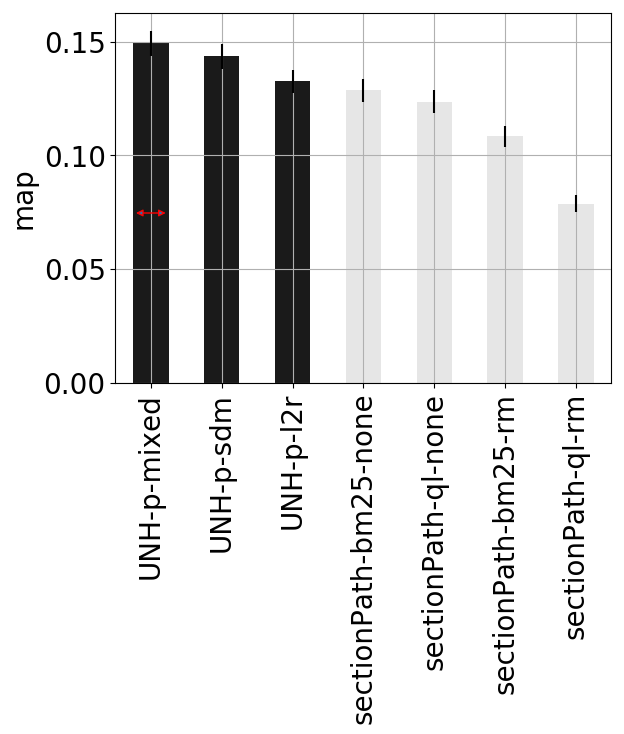
\includegraphics[width=0.5\textwidth]{y1_psg_test.png}}
%     \subfloat[Y2 Test]{ 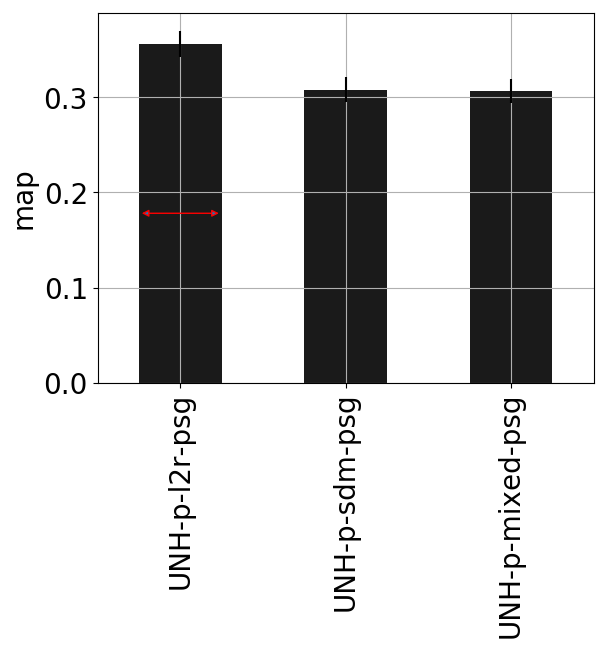
\includegraphics[width=0.5\textwidth]{y2_psg_test.png}}
%     \caption{Performance of passage retrieval methods.}
%     \label{fig:my_label}
% \end{figure}

% \section{Example: Y1 Test Tree Passage}
% 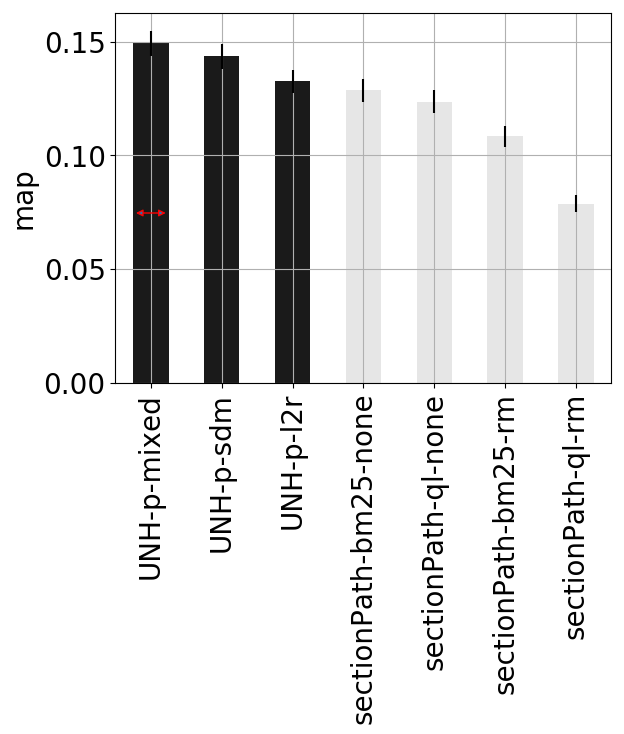
\includegraphics[width=\textwidth]{y1_psg_test.png}

% \section{Example: Y1 Train Tree Passage}
% 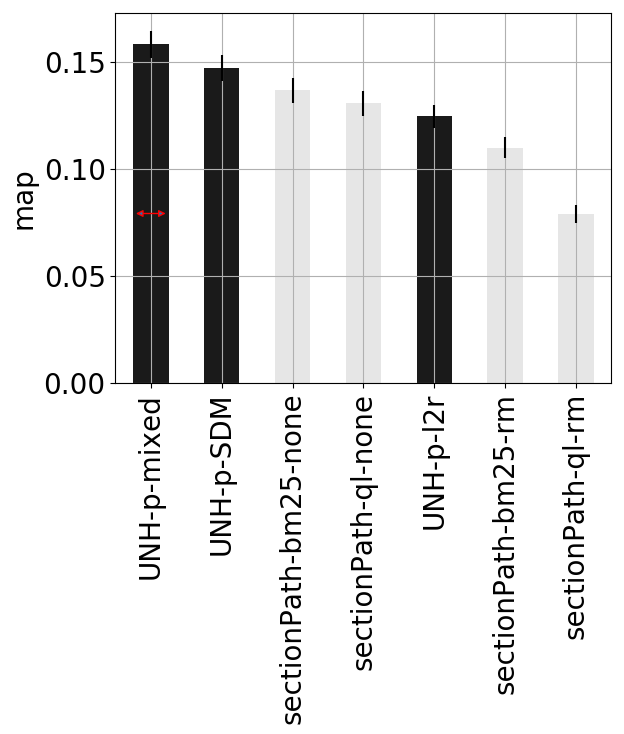
\includegraphics[width=\textwidth]{y1_psg_train.png}

% \section{Example: Y1 Test Tree Entity}
% 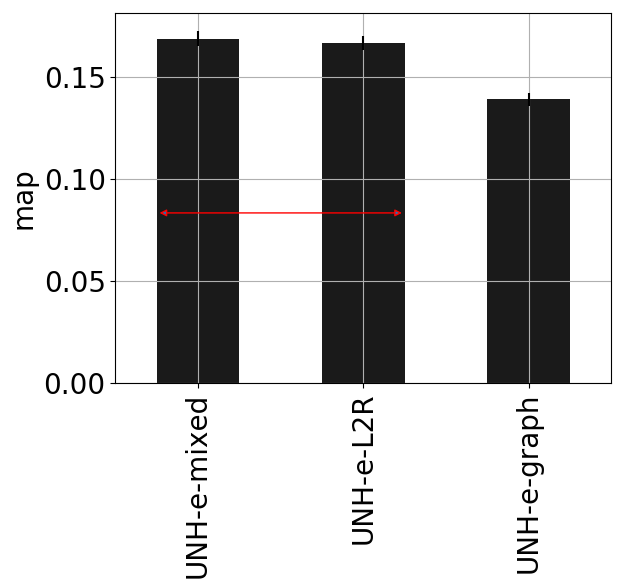
\includegraphics[width=\textwidth]{y1_entity_test.png}

% \section{Example: Y1 Train Tree Entity}
% 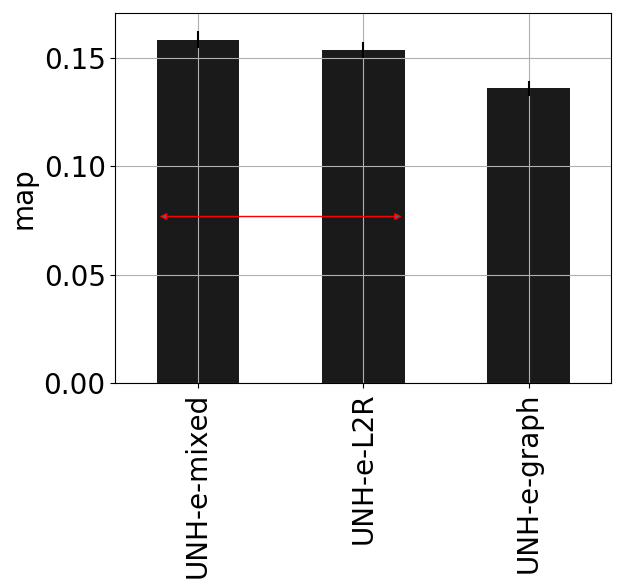
\includegraphics[width=\textwidth]{y1_entity_train.png}

% \section{Example: Y2 Test Entity}
% 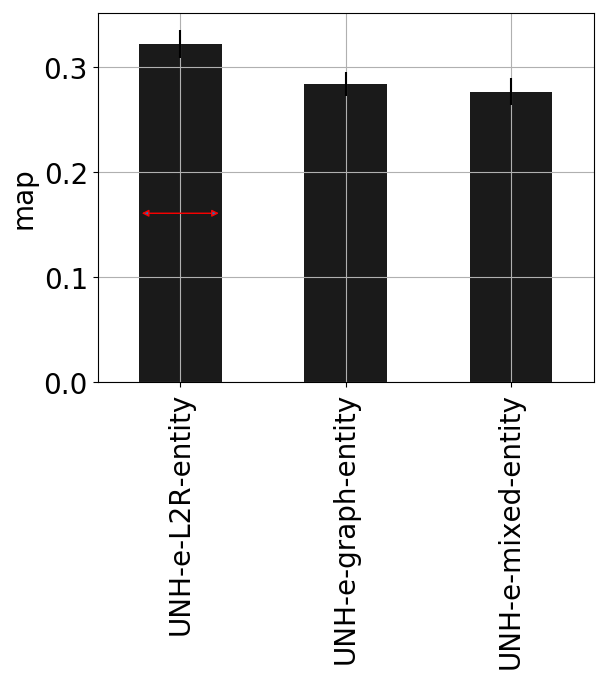
\includegraphics[width=\textwidth]{y2_entity_test.png}

% \section{Example: Y2 Test Passage}
% 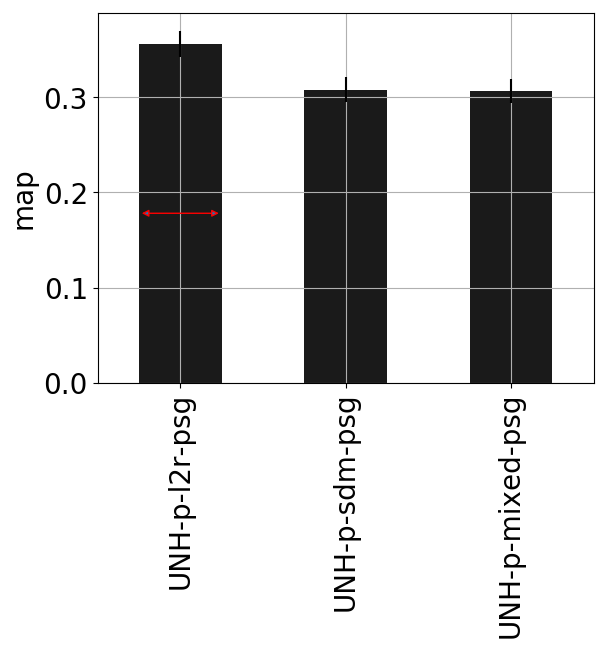
\includegraphics[width=\textwidth]{y2_psg_test.png}



\end{document}

%%
%% End of file `elsarticle-template-1-num.tex'.